% Principal GDZ PPN236018647, native460–463; HKUST461–464.
\clearpage\SourceLeaf{460}\ArithmeticHead{453}{R}{BEMERKUNGEN ZUR TRANSZENDENTEN TRIGONOMETRIE.}
\begingroup\small
\newcommand{\GeomAngle}{\mathord{\vcenter{\hbox{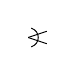
\begin{tikzpicture}[x=.75em,y=.75em,line width=.35pt]\draw (0,.35)--(.9,.65);\draw (0,.35)--(.9,.05);\draw (.15,.8)..controls (.6,.65) and (.6,.05)..(.15,-.1);\end{tikzpicture}}}}}
\HistoricTitle{BEMERKUNGEN.}
\indent Das als Scheda Af bezeichnete Heft enthält Aufzeichnungen der verschiedensten Art, die, wie wiederholte Datierungen zeigen, aus den Jahren 1801 bis 1803 stammen. Da die hier abgedruckten Notizen fast am Ende des Heftes stehen, ist anzunehmen, daß ihre Abfassung in das Jahr 1803 fällt. Neben der Aufzeichnung Nr. 99 des \textit{Tagebuchs}: \textls[120]{In principiis geometriae egregios progressus fecimus}, Br[unovici 1799] Sept., und den Äußerungen in dem Briefe an \textsc{Wolfgang Bolyai} vom 16. Dez. 1799, (Werke VIII, S. 159) bilden die vorstehenden Notizen das älteste Zeugnis für \textsc{Gauss}ens Beschäftigung mit den Grundlagen der Geometrie; sie sind um so wertvoller, als es sich in ihnen um Versuche handelt, einen Zugang zu der \textls[120]{transzendenten Trigonometrie} zu gewinnen, von der \textsc{Gauss} seinem Schüler \textsc{Wachter} bei dessen Besuch im April 1816 erzählt hat (Werke VIII, S. 176).

\indent Die Notiz [I.] enthält einen Ansatz, um für ein rechtwinkliges Dreieck, bei dem der eine spitze Winkel \(\omega\) so klein ist, daß man in den Reihenentwicklungen nach Potenzen von \(\omega\) von den Gliedern dritter und höherer Ordnung absehen darf, Beziehungen zwischen den Seiten und Winkeln zu finden. Es sei also im Dreieck \(ABC\) der Winkel bei \(C\) ein Rechter und der Winkel \(\omega\) bei \(A\) sehr klein: die Kathete \(AC\) werde mit \(\Delta\) bezeichnet. Dann ist in erster Näherung:
\begin{center}
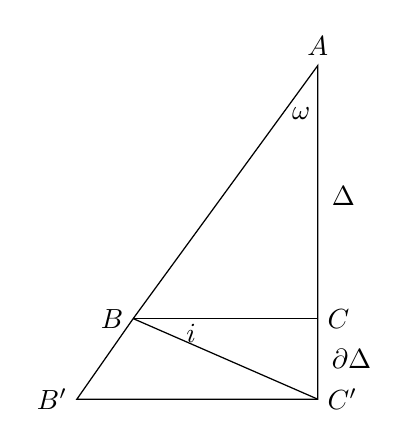
\begin{tikzpicture}[x=.011cm,y=-.011cm,line width=.45pt]
\draw (278,0)--(65,292)--(0,385)--(278,385)--cycle;
\draw (65,292)--(278,292);
\draw (65,292)--(278,385);
\node[above] at (278,0) {$A$};
\node[left] at (65,292) {$B$};
\node[right] at (278,292) {$C$};
\node[left] at (0,385) {$B'$};
\node[right] at (278,385) {$C'$};
\node at (259,55) {$\omega$};
\node[right] at (283,150) {$\Delta$};
\node at (132,309) {$i$};
\node[right] at (283,338) {$\partial\Delta$};
\end{tikzpicture}
\end{center}
\begin{equation}BC=\omega\varphi(\Delta),\tag{1}\end{equation}
\begin{equation}\GeomAngle ABC=90^{0}-\omega-\omega\psi(\Delta),\tag{2}\end{equation}
\noindent wo \(\varphi(\Delta),\ \psi(\Delta)\) noch zu bestimmende Funktionen bedeuten. Die Winkelsumme im Dreieck \(ABC\) ist \(180^{0}-\omega\psi(\Delta)\), also, wenn die Funktion \(\psi(\Delta)\) positiv ist, kleiner als \(180^{0}\). Um die unbekannten Funktionen \(\varphi(\Delta)\) und \(\psi(\Delta)\) zu bestimmen, verlängere man \(AC\) um \(CC'=\partial\Delta\), errichte in \(C'\) auf \(AC'\) das Lot \(C'B'\), das die Verlängerung von \(AB\) in \(B'\) treffe, und ziehe \(BC'\); der Winkel \(CBC'\) werde mit \(i\) bezeichnet. Dann ergibt die Anwendung der Formel (1) auf das Dreieck \(BCC'\):
\begin{equation}\partial\Delta=i\varphi(\omega\varphi(\Delta)).\tag{3}\end{equation}
\noindent Das quergestreifte Dreieck in der Notiz [I.], S. 451 soll auf den \textls[120]{Inhalt} des Dreiecks hinweisen. Dieser ist in der antieuklidischen Geometrie der Abweichung der Winkelsumme von \(180^{0}\) proportional. Mithin wird der Inhalt des Dreiecks \(ABC\) proportional \(\omega\psi(\Delta)\) und daher ist der Inhalt des Vierecks \(BCC'B'\) proportional \(\omega\partial\psi(\Delta)\). Nun ist das Viereck \(BCC'B'\), bis auf Größen höherer Ordnung, doppelt so groß wie das Dreieck \(BCC'\), dessen Inhalt proportional \(i\psi(\omega\varphi(\Delta))\) ist, folglich gilt die Gleichung
\begin{equation}\omega\partial\psi(\Delta)=2i\psi(\omega\varphi(\Delta)).\tag{4}\end{equation}
\noindent Durch Verbindung von (3) und (4) gelangt man zu der Funktionalgleichung
\begin{equation}\psi'(\Delta)=\frac{2\psi(\omega\varphi(\Delta))}{\omega\varphi(\omega\varphi(\Delta))}\mathpunct{\raisebox{.45ex}{.}}\tag{5}\end{equation}
\noindent Um sie zu lösen, setzt \textsc{Gauss}
\begin{equation}\varphi(\Delta)=\chi'(\Delta)\tag{6}\end{equation}
\noindent und denkt sich \(\chi'(\Delta)\) nach Potenzen von \(\Delta\) entwickelt:
\begin{equation}\chi'(\Delta)=\alpha\Delta+\mathinner{\cdotp\cdotp\cdotp},\tag{7}\end{equation}
\clearpage\SourceLeaf{461}\ArithmeticHead{454}{L}{GEOMETRIE. NACHLASS.}
\noindent das konstante Glied fehlt, weil \(\varphi(0)=0\) ist. Jetzt wird nach (5):
\begin{equation}\psi'(\Delta)\{\alpha\omega^2\chi'(\Delta)+\mathinner{\cdotp\cdotp\cdotp}\}=2\psi(\omega\chi'(\Delta)),\tag{8}\end{equation}
\noindent mithin muß die Entwicklung von \(\psi(\Delta)\) nach Potenzen von \(\Delta\) mit einem Gliede \(\beta\Delta^2\) anfangen, und man hat, nach Potenzen von \(\omega\) entwickelnd:
\begin{equation}\psi'(\Delta)\mathbin{.}\alpha\omega^2\chi'(\Delta)+\mathinner{\cdotp\cdotp\cdotp}=2\beta\omega^2(\chi'(\Delta))^2+\mathinner{\cdotp\cdotp\cdotp},\tag{9}\end{equation}
\noindent woraus durch Vergleichung der Koeffizienten von \(\omega^2\) die Schlußformel von \textsc{Gauss} hervorgeht:
\begin{equation}\alpha\psi'(\Delta)=2\beta\chi'(\Delta).\tag{10}\end{equation}

\indent Um die Rechnung zu Ende zu führen, integriere man die Gleichung (10) und substituiere
\begin{equation}\psi(\Delta)=\frac{2\beta}{\alpha}\chi(\Delta)\tag{11}\end{equation}
\noindent in der Funktionalgleichung (5). Indem noch \(\omega\chi'(\Delta)=\xi\) gesetzt wird, geht diese über in die Differentialgleichung
\begin{equation}\xi\chi'(\xi)=2\chi(\xi),\tag{12}\end{equation}
\noindent mithin ist \(\chi(\xi)=\tfrac12\alpha\xi^2\) und
\begin{equation}\varphi(\xi)=\alpha\xi,\quad\psi(\xi)=\beta\xi^2.\tag{13}\end{equation}
\noindent Dabei ist \(\xi=\omega\chi'(\Delta)\). Indem man beachtet, daß von vornherein bei den Entwicklungen nach Potenzen von \(\omega\) von den Gliedern dritter und höherer Ordnung abgesehen wurde, ergibt sich schließlich, daß der Ansatz unter den gemachten Voraussetzungen zu den Gleichungen führt:
\begin{equation}
\left\{\begin{aligned}
\varphi(\Delta)&=\alpha\Delta+\ast+\alpha_3\Delta^3+\mathinner{\cdotp\cdotp\cdotp},\\
\psi(\Delta)&=\ast+\beta\Delta^2+\beta_3\Delta^3+\mathinner{\cdotp\cdotp\cdotp},
\end{aligned}\right.\tag{14}
\end{equation}
\noindent wobei die Koeffizienten \(\alpha,\ \alpha_3,\mathinner{\ldotp\ldotp\ldotp};\ \beta,\ \beta_3,\mathinner{\ldotp\ldotp\ldotp}\) \textls[120]{unbestimmt} bleiben.

\indent \textsc{Gauss} hat neben die letzten Formeln der Notiz [I.] geschrieben:
\[\varphi(\Delta)=\sin\Delta.\]
\noindent In der Tat wird die Funktionalgleichung (5) durch diese Annahme für \(\varphi(\Delta)\) in Verbindung mit
\[\psi(\Delta)=-(1-\cos\Delta)\]
\noindent erfüllt, wenn, den Voraussetzungen entsprechend, \(\sin(\omega\sin\Delta)\) durch \(\omega\sin\Delta\) und \(\cos(\omega\sin\Delta)\) durch \(1-\tfrac12\omega^2\sin^2\Delta\) ersetzt werden darf, und man wird so auf die in der \textls[120]{sphärischen Trigonometrie} geltenden Gleichungen geführt.

\indent Im Unterschied gegen die Notiz [I.] wird in der Notiz [III.] ein Ansatz versucht, bei dem \(\omega\) einen beliebigen spitzen Winkel bezeichnet. Einen Übergang hierzu bildet die kurze Notiz [II.], in der bereits \(\omega\varphi(\Delta)\) und \(\omega\psi(\Delta)\) durch \(\varphi(\omega,\Delta)\) und \(\psi(\omega,\Delta)\) ersetzt werden. Jedoch gilt die Gleichung
\[\frac{\partial\varphi(\omega,\Delta)}{\partial\Delta}=\psi(\omega,\Delta),\]
\noindent wie man sich leicht überzeugt, nur für kleine Winkel \(\omega\) im Sinne der Notiz [I.].

\indent In der Aufzeichnung [III.] handelt es sich um ein rechtwinkliges Dreieck mit dem spitzen Winkel \(\omega\), bei dem die Hypotenuse mit \(\Delta\) bezeichnet wird; die Katheten heißen \(\varphi(\omega,\Delta)\) und \(\chi(\omega,\Delta)\), der andere spitze
\clearpage\SourceLeaf{462}\ArithmeticHead{455}{R}{BEMERKUNGEN ZUR TRANSZENDENTEN TRIGONOMETRIE.}
\noindent Winkel wird gleich \(90^{0}-\psi(\omega,\Delta)\) gesetzt. Es ist also in der Figur:
\begin{center}
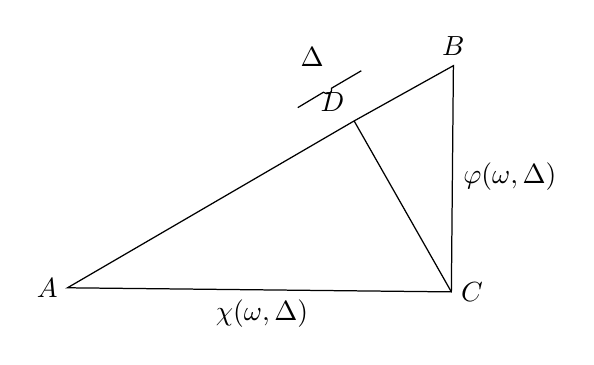
\begin{tikzpicture}[x=.013cm,y=-.013cm,line width=.45pt]
\draw (0,217)--(280,54)--(377,0)--(375,221)--cycle;
\draw (280,54)--(375,221);
\draw (225,41)--(250,26)..controls (254,29) and (259,27)..(258,22)--(287,5);
\node[left] at (0,217) {$A$};
\node[above] at (377,0) {$B$};
\node[right] at (375,221) {$C$};
\node[above left] at (280,54) {$D$};
\node[above] at (239,10) {$\Delta$};
\node[right] at (377,108) {$\varphi(\omega,\Delta)$};
\node[below] at (190,219) {$\chi(\omega,\Delta)$};
\end{tikzpicture}
\end{center}
\begin{equation}
\left\{\begin{aligned}BC&=\varphi(\omega,\Delta),\\AC&=\chi(\omega,\Delta),\\\GeomAngle ABC&=90^{0}-\psi(\omega,\Delta).\end{aligned}\right.\tag{I}
\end{equation}

\indent Um Beziehungen zwischen den Funktionen \(\varphi(\omega,\Delta),\ \chi(\omega,\Delta)\) und \(\psi(\omega,\Delta)\) zu gewinnen, fälle man von \(C\) das Lot \(CD\) auf die Hypotenuse \(AB\) und betrachte die rechtwinkligen Teildreiecke \(ACD\) und \(BCD\). Zunächst wird im Dreieck \(ACD\):
\begin{equation}
\left\{\begin{aligned}CD&=\varphi(\omega,\chi(\omega,\Delta)),\\AD&=\chi(\omega,\chi(\omega,\Delta)),\\\GeomAngle ACD&=90^{0}-\psi(\omega,\chi(\omega,\Delta)).\end{aligned}\right.\tag{II}
\end{equation}
\noindent Mithin ist im Dreieck \(BCD\) der Winkel \(BCD\) gleich \(\psi(\omega,\chi(\omega,\Delta))\) und daher:
\begin{equation}
\left\{\begin{aligned}
DB&=\varphi\{\psi(\omega,\chi(\omega,\Delta)),\varphi(\omega,\Delta)\},\\
CD&=\chi\{\psi(\omega,\chi(\omega,\Delta)),\varphi(\omega,\Delta)\},\\
\GeomAngle CBD&=90^{0}-\psi\{\psi(\omega,\chi(\omega,\Delta)),\varphi(\omega,\Delta)\}.
\end{aligned}\right.\tag{III}
\end{equation}
\noindent Nun ist \(AD+DB=AB,\ \GeomAngle CBD=\GeomAngle ABC\) und es müssen die beiden für \(CD\) gefundenen Werte übereinstimmen. Hieraus folgen die Funktionalgleichungen:
\begin{equation}
\left\{\begin{aligned}
\Delta&=\chi(\omega,\chi(\omega,\Delta))+\varphi\{\psi(\omega,\chi(\omega,\Delta)),\varphi(\omega,\Delta)\},\\
\psi(\omega,\Delta)&=\psi\{\psi(\omega,\chi(\omega,\Delta)),\varphi(\omega,\Delta)\},\\
\varphi(\omega,\chi(\omega,\Delta))&=\chi\{\psi(\omega,\chi(\omega,\Delta)),\varphi(\omega,\Delta)\}.
\end{aligned}\right.\tag{IV}
\end{equation}

\indent Um aus ihnen die Funktionen \(\varphi,\chi,\psi\) zu bestimmen, entwickelt \textsc{Gauss} nach Potenzen von \(\omega\) und setzt:
\begin{equation}
\left\{\begin{aligned}
\varphi(\omega,\Delta)&=\omega f(\Delta)+\omega^2 f'(\Delta)+\omega^3 f''(\Delta)+\mathinner{\cdotp\cdotp\cdotp},\\
\chi(\omega,\Delta)&=\Delta+\omega g(\Delta)+\omega^2 g'(\Delta)+\omega^3 g''(\Delta)+\mathinner{\cdotp\cdotp\cdotp},\\
\psi(\omega,\Delta)&=\omega+\omega^2 h'(\Delta)+\omega^3 h''(\Delta)+\mathinner{\cdotp\cdotp\cdotp};
\end{aligned}\right.\tag{V}
\end{equation}
\noindent die Striche bedeuten hier nicht wie in der Notiz [I.] Ableitungen nach \(\Delta\), sondern sind als Indizes aufzufassen. Warum als Anfangsglieder der Entwicklungen \(\omega f(\Delta),\ \Delta\) und \(\omega\) angenommen sind, ergibt die Figur, indem man zur Grenze für \(\omega=0\) übergeht; vergl. auch die Gleichung (2) zur Notiz [I.].

\indent In der Scheda Af folgen noch einige flüchtig hingeworfene Zeilen, die zeigen, daß \textsc{Gauss} die Entwicklungen (V) in die Gleichungen (IV) eingesetzt hat, aber nicht zur Bestimmung der Koeffizienten vorgedrungen ist; ihr Abdruck erschien nicht erforderlich. Dagegen verdient erwähnt zu werden, daß \textsc{Gauss} dazwischen die Formel
\[
\operatorname{Arctang}(\cos\omega\mathbin{.}\operatorname{tang}\Delta)=\cos\omega\mathbin{.}\operatorname{t}[\operatorname{ang}\Delta]-\tfrac13\cos\omega^3\mathbin{.}\operatorname{t}[\operatorname{ang}\Delta^3+\mathinner{\cdotp\cdotp\cdotp}]
\]
\noindent vermerkt hat, deren linke Seite in der sphärischen Trigonometrie der Ausdruck für die Funktion \(\chi(\omega,\Delta)\) ist.

\indent Die Notiz [IV.] enthält einen anderen Ansatz, bei dem nur zwei zu bestimmende Funktionen auftreten. Um den Punkt \(O\) werde der Kreis mit dem Halbmesser \(\Delta\) beschrieben. Es seien \(AB\) und \(BC\)
\clearpage\SourceLeaf{463}\ArithmeticHead{456}{L}{GEOMETRIE. NACHLASS.}
\noindent zwei Sehnen mit den Zentriwinkeln \(a\) und \(b\). Von \(O\) fälle man auf \(AB\) das Lot \(OD\), auf \(AC\) das Lot \(BF\). Wenn dann die Funktionen \(\varphi(\omega,\Delta)\) und \(\psi(\omega,\Delta)\) dieselbe Bedeutung haben, wie in der Notiz [III.], so ist
\begin{center}
\begin{tikzpicture}[x=.013cm,y=-.013cm,line width=.45pt]
\draw (0,0)--(0,464)--(467,464);
\draw (0,0)--(209,133)--(422,268)--(445,366)--(467,464);
\draw (0,0)..controls (190,0) and (342,95)..(422,268)..controls (455,342) and (467,418)..(467,464);
\draw (0,0)--(346,345)--(467,464);
\draw (0,464)--(209,133);
\draw (0,464)--(422,268);
\draw (0,464)--(445,366);
\draw (422,268)--(346,345);
\node[above] at (0,0) {$A$};
\node[above right] at (422,268) {$B$};
\node[below] at (467,464) {$C$};
\node[above right] at (209,133) {$D$};
\node[right] at (460,366) {$E$};
\node[below left] at (346,345) {$F$};
\node[below] at (0,464) {$O$};
\node[below] at (210,467) {$\Delta$};
\node[inner sep=0pt] at (25,397) {$\tfrac12 a$};
\node[inner sep=0pt] at (58,418) {$\tfrac12 a$};
\node[inner sep=0pt] at (117,434) {$\tfrac12 b$};
\node[inner sep=0pt] at (125,453) {$\tfrac12 b$};
\end{tikzpicture}
\end{center}
\[
\begin{gathered}
AB=2\varphi(\Delta,\tfrac12 a),\quad BC=2\varphi(\Delta,\tfrac12 b),\\
\GeomAngle OAD=\GeomAngle OBD=90^{0}-\psi(\Delta,\tfrac12 a),\\
\GeomAngle OBE=\GeomAngle OCE=90^{0}-\psi(\Delta,\tfrac12 b),\\
\GeomAngle OAF=\GeomAngle OCF=90^{0}-\psi(\Delta,\tfrac12(a+b))
\end{gathered}
\]
\noindent und daher
\[
\begin{aligned}
\GeomAngle BAF&=\psi(\Delta,\tfrac12(a+b))-\psi(\Delta,\tfrac12 a),\\
\GeomAngle BCF&=\psi(\Delta,\tfrac12(a+b))-\psi(\Delta,\tfrac12 b).
\end{aligned}
\]
\noindent Mithin wird im Dreieck \(BAF\):
\[BF=\varphi\{2\varphi(\Delta,\tfrac12 a),\ \psi(\Delta,\tfrac12(a+b))-\psi(\Delta,\tfrac12 a)\}\]
\noindent und im Dreieck \(BCF\):
\[BF=\varphi\{2\varphi(\Delta,\tfrac12 b),\ \psi(\Delta,\tfrac12))-\psi(\Delta,\tfrac12 b)\}.\]
\noindent Dies ist die erste Funktionalgleichung des Textes. Die zweite erhält man aus der doppelten Zerlegung des Winkels \(ABC\):
\[\GeomAngle ABC=\GeomAngle ABF+\GeomAngle CBF=\GeomAngle OBD+\GeomAngle OBE.\]

\indent Die weiteren Rechnungen brechen sogleich wieder ab. \textsc{Gauss} hat noch für \(\varphi(\Delta,a)\) und \(\psi(\Delta,a)\) die Ausdrücke hingeschrieben, die in der sphärischen Trigonometrie gelten, nämlich
\[
\begin{aligned}
\varphi(\Delta,a)&=\Delta\sin a-\tfrac16\Delta^3\sin a\mathbin{.}\cos a^2+\mathinner{\cdotp\cdotp\cdotp},\\
\psi(\Delta,a)&=a-\tfrac12\Delta\Delta\sin a\mathbin{.}\cos a+\mathinner{\cdotp\cdotp\cdotp}.
\end{aligned}
\]

\indent Auf weitere Untersuchungen über die transzendente Trigonometrie deuten einige Figuren auf S. 71 der Scheda, von denen eine hier wiedergegeben sei. Was damit beabsichtigt ist, hat sich nicht feststellen lassen. Es ist bemerkenswert, daß die Werke VIII, S. 255—257 abgedruckte Notiz, in der \textsc{Gauss} eine Herleitung der transzendenten Trigonometrie gibt, ebenfalls auf geometrischen Konstruktionen und daraus folgenden Relationen für zwei unbekannte Funktionen beruht. Man vergleiche auch den in der zweiten Abteilung dieses Bandes abgedruckten Aufsatz »\textsc{Gauss} als Geometer«.
\begin{center}
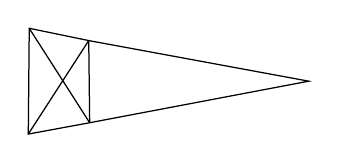
\begin{tikzpicture}[x=.012cm,y=-.012cm,line width=.45pt]
\draw (0,0)--(63,13)--(296,56)--(64,100)--(-1,112)--cycle;
\draw (63,13)--(64,100);
\draw (0,0)--(64,100);
\draw (-1,112)--(63,13);
\end{tikzpicture}
\end{center}
\par\noindent\hfill\textsc{Stäckel}.
\ClosingRule
\par\endgroup\ArithmeticHead{456}{L}{GEOMETRIE. NACHLASS.}
